\documentclass[a4paper]{article}%

\usepackage[english]{babel}%
\usepackage[utf8]{inputenc}%
\usepackage[T1]{fontenc} %

\usepackage{graphicx}%
\usepackage{xspace}%

\usepackage{amsmath}
\usepackage{amsfonts}
\usepackage{amssymb}

\usepackage{tikz}
\usetikzlibrary{arrows}

\usepackage{xcolor,colortbl}

\usepackage[margin=2.5cm]{geometry}

\usepackage{caption}
\usepackage{subcaption}
\usepackage{float}  % H option for figures

\DeclareMathOperator{\E}{E}
\DeclareMathOperator{\Cod}{Cod}
\newcommand{\CodSk}{\overset{\sim}{\Cod}}


\begin{document}

\title{Project IRESI}

\author{Simon Bihel, Florestan De Moor \\ ENS Rennes, Computer Science Department, 1st year}

\date{November 22, 2015}

\maketitle

\begin{abstract}
	In this report we present our work on the project of the course IRESI. We will first explain how we implemented the \texttt{SketchMin} algorithm, which is a metric used to detect DDoS. We coded this using the Python 3 language. We will then compare the results of the algorithm to exact values.
\end{abstract}


\section{DDoS and server security}

A DDoS (Distributed Denial of Service) attack is nowadays a well-known issue : it consists of sending a huge number of requests to a server, so that it crashes, and therefore to make it unavailable for the other users. The requests are sent to the server by the router, which receives data streams. If the attack is concentrated in a single stream, it is easy do detect it.

\begin{figure}[H]
	\center
	\begin{tikzpicture}[->,>=stealth',shorten >=1pt,auto,node distance=4.cm]
	
	  \node (A){
\includegraphics[scale=0.2]{computer.png}};
	  \node (B) [right of=A] {
\includegraphics[scale=0.1]{router.png}};
	  \node (C) [right of=B] {
\includegraphics[scale=0.2]{server.png}};
	
	  \path
	(A) edge [draw=red, line width=0.5mm] node {Packets} (B)
	(B) edge [draw=purple, line width=0.5mm] node {} (C);
	
	\end{tikzpicture}
	\caption{\scriptsize One user sending requests to a server, through the router}
\end{figure}

However, if the attack is scattered among several streams, it is much more difficult to detect it.

\begin{figure}[H]
	\center
	\begin{tikzpicture}[->,>=stealth',shorten >=1pt,auto]
	
	\node (A){
\includegraphics[scale=0.2]{computer.png}};
	\node (B) [right of=A, node distance=4.cm] {
\includegraphics[scale=0.1]{router.png}};
	\node (C) [right of=B, node distance=4.cm] {
\includegraphics[scale=0.2]{server.png}};
	\node (D) [below of=A, node distance=2.3cm]{
\includegraphics[scale=0.2]{computer.png}};
	\node (E) [above of=A, node distance=2.3cm]{
\includegraphics[scale=0.2]{computer.png}};
	
	  \path
	(A) edge [draw=red, line width=0.5mm] node {Packets} (B)
	(D) edge [draw=red, line width=0.5mm] node {Packets} (B)
	(E) edge [draw=red, line width=0.5mm] node {Packets} (B)
	(B) edge [draw=purple, line width=1.5mm] node {} (C);
	
	\end{tikzpicture}
	\caption{\scriptsize Three users sending requests to a server, through the router}
\end{figure}

\paragraph{}That's why the following method was implemented : the router receives different data streams, and calculates for each peer a correlation indicator which is the codeviance of the frequency vectors corresponding to the streams. The codeviance formulas are presented below in section \textbf{2.2}. Once this was computed, it becomes possible to determine if an attack is happening or not, by analysing the codeviance values.

\begin{figure}[H]
	
	\begin{center}\begin{tabular}{|c|c|c|c|c|c|c|c|c|c|c|c|c|c|c|c|c|c|c|c|}
		\hline
		~ & ~ & \cellcolor{purple}~ & ~ & \cellcolor{purple}~ & ~ & ~ & \cellcolor{purple}~ & ~ & ~ & \cellcolor{purple}~ & ~ & ~ & ~ & ~ & ~ & ~ &\cellcolor{purple}~ & ~ & ~ \\
		\hline
	\end{tabular}\end{center}
		
	\begin{center}\begin{tabular}{|c|c|c|c|c|c|c|c|c|c|c|c|c|c|c|c|c|c|c|c|}
		\hline
		\cellcolor{purple}~ & ~ & ~ & ~ & \cellcolor{purple}~ & ~ & \cellcolor{purple}~ & ~ & ~ & ~ & \cellcolor{purple}~ & ~ & ~ & ~ & \cellcolor{purple}~ & ~ & ~ & ~ & \cellcolor{purple}~ & ~ \\
		\hline
	\end{tabular}\end{center}
	\caption{\scriptsize Correlation between two data streams}
\end{figure}

\paragraph{}Nevertheless, the stream sizes are huge, we can't afford to calculate the precise codeviance. The \texttt{SketchMin} algorithm is an easier way to calculate an estimated codeviance using hashing functions in which precision is controlled by a set of parameters ($\varepsilon, \delta)$. We will present in next section how we implemented it using the Python 3 language. We will then compare its results with exact values in section \textbf{3}, by running it with real and randomly generated data traces.


\section{Programming the SketchMin algorithm}

For the detection we need to first select the entries to then apply the algorithm that will produce the material in which we will find whether or not there is an attack.

\subsection{Extracting information from data traces}


In data traces, each line corresponds to a request made to the server. To extract a certain kind information, like the source of a request, there is just to go through each line which represent a line. And each time split the line based on white-spaces and extract a certain entry. The entries are put in a list, and if needed are converted to integers without losing the fact that some entries are identical and others different. This can be done by creating a list of the distinct elements and the converting each element of the original list to the its index in the distinct elements list.
% TODO dernière phrase pas claire

\paragraph{}This process has to be extended to the extraction of multiple traces in a single time because what we want in the end is eventually find correlation between multiple traces. This was the most difficult part of the work. Same entries must be converted to the same integer, even if they're not in the same trace. We were first making the extraction considering only one trace, but we finally had to make the extraction of all traces at once. To do that the distinct elements list has just to be shared between the multiple extractions. And so, identical requests can be correlated after applying the \texttt{SketchMin} algorithm and act in reaction.

\subsection{Computing the codeviance}

First, we implemented two functions to compute the average, and codeviance of an array. To do this, we browse the array, and use the following formulas :
	\[ \E(X) = \frac{1}{|X|} \sum\limits_{x_i \in X} x_i \]
	\[ \Cod(X,Y) = \E(XY) - \E(X)\E(Y) \]
	
\paragraph{}We have in entry a data trace $D$, and precision parameters $(\varepsilon, \delta)$. We start by defining the following constants :
	\[ k =\left\lceil \frac{1}{\varepsilon} \right\rceil \]
$k$ is the number of partitions we will create.
	\[ t = \left\lceil \log(\frac{1}{\delta}) \right\rceil \]
$t$ is the number of hashing functions we will consider.
	
\paragraph{}The data trace has integers values which stand between $0$ and $u$. We have to define $t$ universal hashing functions $h_i$ :
	\[ h_i(x) = ((a_ix+b_i) \mod u) \mod k \quad \forall i \in \lbrace 1 \ldots t \rbrace \]
where $a_i, b_i$ are randomly generated in $\lbrace 1 \dots t-1 \rbrace$ for $a_i$, and $\lbrace 0 \ldots t-1 \rbrace$ for $b_i$.

\paragraph{}We can then create the partitions, and we get a matrix $R_{0 \leq i \leq t-1, 1 \leq j \leq k}$ where 
 	\[ R_{i,j} = \# \lbrace x \in D : h_i(x) = j \rbrace \]
 	
\paragraph{}We can now create a function that receives two data traces. It calculates the $R$ matrfor both trace, and then computes the codeviance :
	\[ \CodSk(D_1, D_2) = \underset{0 \leq i \leq t-1}{\min} \Cod(R_1[i], R_2[i]) \]
where $R[i]$ is the line $i$ of the matrix.

\paragraph{}We can then create the full codeviance matrix $C_{1 \leq i,j \leq p}$ when we have $p$ data traces :
	\[ C_{i,j} = \CodSk(D_i, D_j) \quad \forall i,j \in \lbrace 1 \ldots p \rbrace \]
We can notice that the codeviance is symmetrical (i.e. $\Cod(X,Y) = \Cod(Y,X)$). That's why only $p(p+1)/2$ computations are made to create this matrix (instead of $p^2$).

\paragraph{}Once we calculated this matrix, we can plot it in 3D to have a visual result. To do this, we used the packages \texttt{numpy} and \texttt{matplotlib} from the Python library.

\paragraph{}This is one of the reasons why we chose to program this algorithm using the Python 3 language : there are a lot of libraries that enable to create a visual plotting very easily. It makes it much easier to test the program, as we will see in next section. Another reason is that the Python language is very simple, with an intuitive syntax. It also deals with reading files quite well, and this was important to extract information from the traces in an effective way.



\section{Experimental results}

To evaluate the correctness of the algorithm, we just need to see if the results have the same appearance than the real values, with possibly a different scale.

\subsection{Real data traces}


For the real traces, we used the file-names as entries for the algorithm, after converting them to integer by simply matching the index of the distinct elements. We used file-names because the calgaryaccess traces didn't really have an entry for the sources of the requests, and we wanted a consistent information extraction over the multiple traces to eventually find correlations. Here are the rest of the parameters for the experiment :


\begin{itemize}
	\item $\varepsilon = 0.001$ which means $k = 1000$ partitions
	\item $\delta = 0.001$ which means $t = 7$ hashing functions
\end{itemize}

In the figure~\ref{ref:exp_real} we can see the result of the experiment where the result of the algorithm is close to the original. Both chart are plotted with a logarithmic scale.


\begin{figure}[H]
	\center
	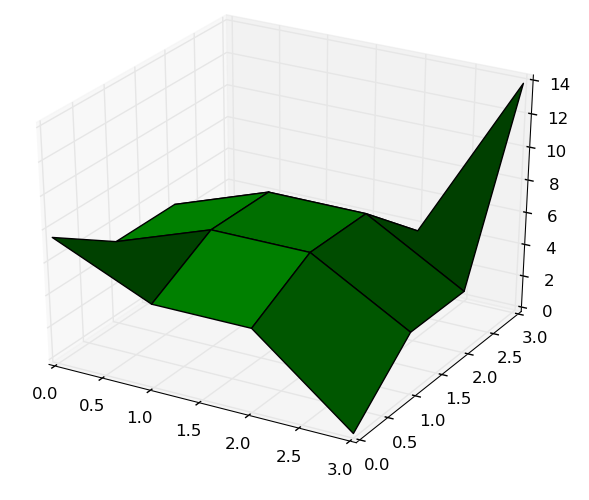
\includegraphics[scale=0.35]{realtests_real1.png}
	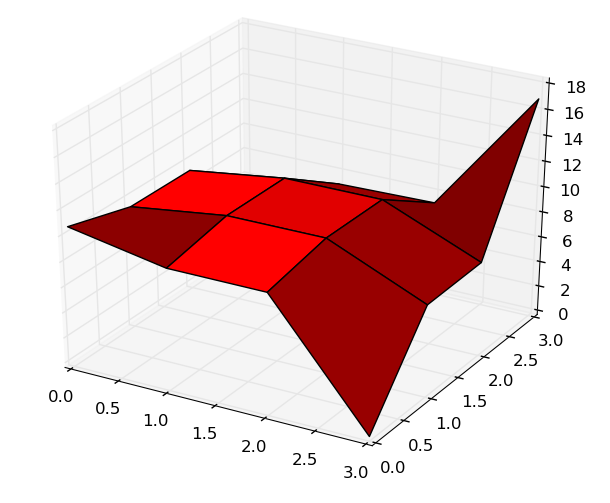
\includegraphics[scale=0.35]{realtests_sketchmin1.png}
	\caption{\footnotesize Codeviance matrix of real data traces: \\ real one (green) - calculated with \texttt{SketchMin} algorithm (red)}
	\label{ref:exp_real}
\end{figure}



\subsection{Generated data traces}


We generated artificial data traces using some probabilistic laws. These traces were generated using the package \texttt{numpy.random} from the Python library. Here are the parameters of this experiment, and the list of the traces we generated :
\begin{itemize}
	\item size of the traces : $size = 10 000$
	\item integers values are generated between $0$ and $u = 100$
	\item $\varepsilon = 0.1$ which means $k = 10$ partitions
	\item $\delta = 0.001$ which means $t = 7$ hashing functions
\end{itemize}

\begin{center}
	\begin{tabular}{|c|c|c|}
		\hline
		 & Probabilistic laws & Parameters \\
		 \hline
		Trace 0 & Uniform & \\
		Trace 1 & Zipfian & $\alpha = 2$ \\
		Trace 2 & Zipfian & $\alpha = 3$ \\
		Trace 3 & Zipfian & $\alpha = 4$ \\
		Trace 4 & Zipfian & $\alpha = 5$ \\ 
		Trace 5 & Zipfian & $\alpha = 6$ \\
		Trace 6 & Poisson & $\lambda = u/(2)$ \\
		Trace 7 & Poisson & $\lambda = u/(2^2)$ \\
		Trace 8 & Poisson & $\lambda = u/(2^3)$ \\
		Trace 9 & Poisson & $\lambda = u/(2^4)$ \\
		Trace 10 & Poisson & $\lambda = u/(2^5)$ \\
		Trace 11 & Binomial & $p = 0.42$ \\
		Trace 12 & Negative Binomial & $p = 0.42$ \\
		\hline
	\end{tabular}
\end{center}


We calculated the real codeviance matrix, and we applied the \texttt{SketchMin} algorithm. Here are the results we got in figure~\ref{ref:exp_artificial} below. We can notice that the two shapes are really similar, though the scales are different.

\begin{figure}[H]
	\centering
	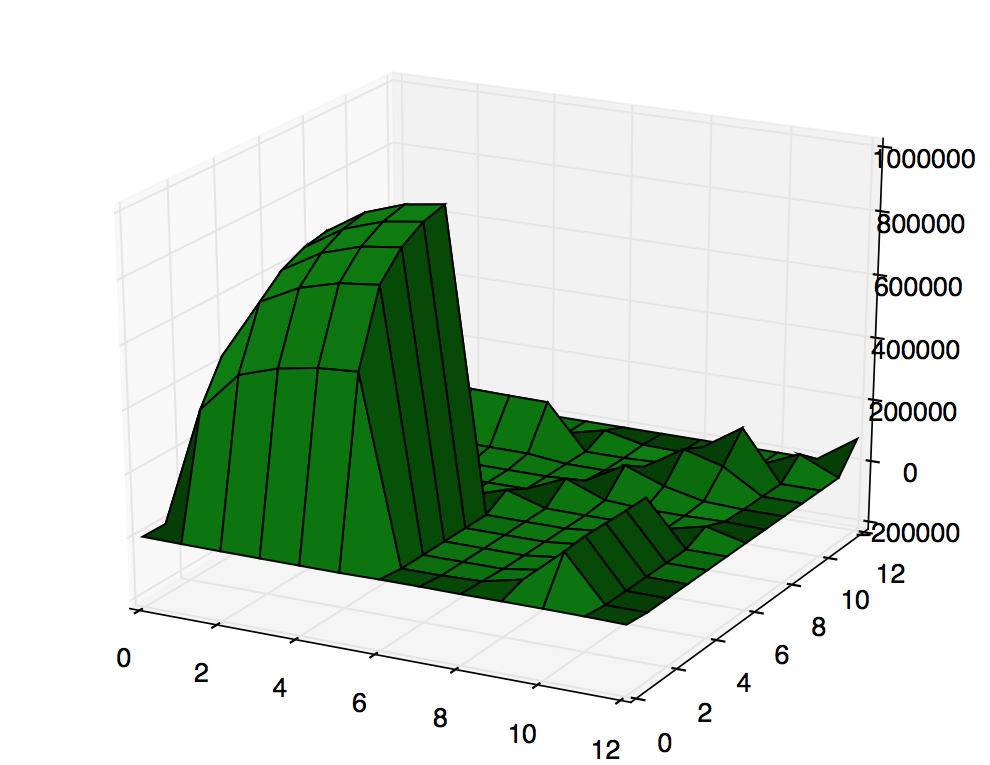
\includegraphics[scale=0.23]{generated_real.png}
	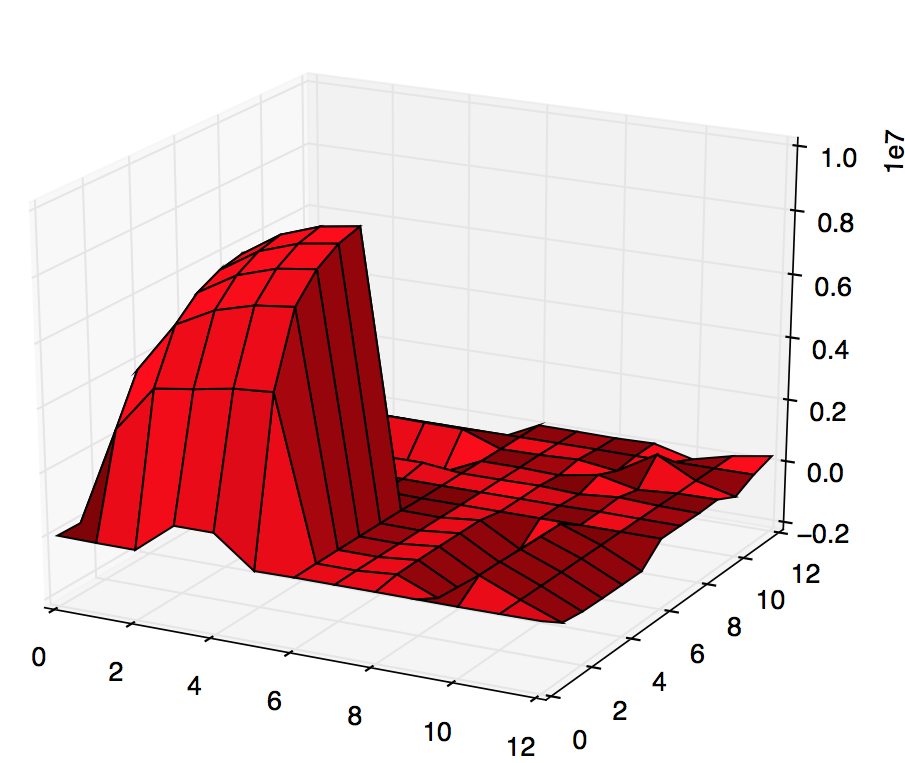
\includegraphics[scale=0.23]{generated_sk.png}
	\caption{\footnotesize Codeviance matrix of generated data traces:\\real one (green) - calculated with \texttt{SketchMin} algorithm (red)}
	\label{ref:exp_artificial}
\end{figure}


\section*{Conclusion}
% TODO
% Simon / Florestan
% results look like exact entries
% what next ? -> find the right parameter to detect a false (=vicious) pike of activity, empirical learning
% what next ? -> put in concurrency the seperate codeviance computings
% chat next ? -> only calculating on a total trace, what about a moving window -> from slide 57 of CM3, with buffers

\clearpage

\end{document}